%% Regular, article-style document with 12pt font and A4 sized paper
\documentclass[12pt,a4paper]{article}

%% UTF-8 support
\usepackage[utf8]{inputenc}

%% Basic packages for formulas, symbols, etc
\usepackage{amsmath}
\usepackage{amsfonts}
\usepackage{amssymb}
\usepackage{multirow}

%% Clean paragraph spacing
\usepackage{parskip}

%% Use 1 inch margins
\usepackage{fullpage}

%% Hyperlink support
\usepackage{hyperref}

%% Support for wrapped images
\usepackage{wrapfig}

%% Image support
\usepackage{graphicx}

%% For description sections (indentable lists)
\usepackage{enumitem}

%% Font improvements
\usepackage[T1]{fontenc}
\usepackage{lmodern}

%% Custom template to create todo notes. This is a red framed box that contains
%% wrapped, bold, red text.
\usepackage{xcolor}
\newcommand\todonote[1]{{\color{red}\fbox{\parbox{\dimexpr\linewidth-2\fboxsep-2\fboxrule}{\textit\large{\textbf{TODO: #1}}}}}}

%% Custom template for paragraphs in tables, which don't leave spaces between
%% paragraphs. Add this to the end of a paragraph to force a nice little space.
\newcommand\tablepar{\vspace{0.25cm}\newline}

%% Header and footer styles (page number centered at the bottom)
\usepackage{fancyhdr}
\usepackage{lastpage}

%% Makes the tables break over multiple pages. If you don't like this
%% behavior, remove this line and replace all instances of "longtable"
%% with "tabular"
\usepackage{longtable}

\begin{document}

%% No page numbering until we get to the main section
\pagenumbering{gobble}

%% Title page
\begin{titlepage}
	\vspace*{\fill}
		\begin{center}
			{\Large{\textbf{File Backup and Management System}}} \\
			\bigskip
			{\Large{\textbf{Milestone 6}}} \\
			\bigskip
			\bigskip
			\bigskip
			\bigskip
			{\Large{\textbf{Submitted by: } \\
			Group 06}} \\
			\begin{description}[labelindent=5cm]
				\item Mike Hoffert - mlh374
				\item Syed Ahsan Rizvi - sar457
				\item Hattan Alsharif - haa775
				\item Da Tao - dat293
				\item Michael Butler - mdb815
			\end{description}
			\bigskip
			\bigskip
			\bigskip
			\bigskip
			\Large{\textbf{Date:} \\
			November 23, 2013}
		\end{center}
	\vspace*{\fill}
\end{titlepage}
\clearpage

%% Abstract
\begin{abstract}
The \textit{File Backup or Management System}, henceforth referred to as \textbf{FBMS}, is a system for backing up files while maintaining revisions. FBMS monitors the file operations that take place within the folder that the user wants to backup (called the "live directory"). Not only are file changes copied to the specified backup directory, but revisions (the instance of the file at a given time) are stored in a database, allowing the program to restore the file's state from any point of time.

FBMS works on all locally accessible drives, including external drives and network drives. The revisioning creates a patch file for plain text, keeping file size down. For binary files, the entire file is stored as the revision. This revisioning ensures not only are the user's files safe, but erroneous changes can be reverted.

FBMS has a focus on ease of use. A wizard guides the user through the setup, where the backup and live directories are chosen. With that complete, the program will run in the background and needs no user interaction until the use desires to restore or view files from the backup.

\todonote{Alsharif, Tao, Butler, and Rizvi. Review and revise}
\end{abstract}
\clearpage

%% Table of contents
\setcounter{tocdepth}{2}
\tableofcontents
\clearpage

%% Page numbering starts here. We begin using the "fancy" page style to allow us to
%% have "page x of y" in the footer. We also have to remove the default headers.
\pagenumbering{arabic}
\pagestyle{fancy}
\fancyhf{} %% Remove the default text
\renewcommand{\headrulewidth}{0pt} %% Remove the header bar
\cfoot{\thepage\ of \pageref{LastPage}} %% New footer content

%% Various content sections. \section denotes level 1 headers, \subsection is level 2,
%% \subsubsection is level 3. All sections automatically added to ToC.
\section{Introduction}

\subsection{System description}
FBMS is an automated backup and revision program. The user specifies a folder that they want to keep backed up (the "live directory") and the location to store the backup (the "backup directory"). The program automatically copies changes in the live directory to the backup directory. Revisions are automatically created by creating "patch" files for every change.

Thus, not only is the user's data backed up, but older versions of the data are also backed up. FBMS can be thought of as a hybrid of a local-only Dropbox\cite{dropbox} and a version control system. While it's not as customizable as a version control system like SVN\cite{svn} or git\cite{git}, FBMS is easy to use and runs in the background without the need for user interaction.

FBMS backs up and revisions both plain text and binary files. A maximum file size to backup can be set. It's also possible to configure the system to remove revisions older than a certain date.

\subsection{Business case}
FBMS helps ensure the user's files are safely backed up without having to depend on limited cloud-based services or the complexity of programs like SVN\cite{svn}. Programs like Dropbox\cite{dropbox} keep revisions of files, but are limited in their ability to do so. FBMS removes these shackles, limiting you only by your hard drive capacity. FBMS currently supports multiple drive systems, including network drives, filling in the blanks of programs like Dropbox, which are online only.

FBMS differs itself from other backup systems in how it doesn't just backup files, but keeps revisions for safety. FBMS is targeted as the semi-casual audience, who know enough to understand the need for backups, but don't want to use a version control system (or perhaps don't like using such systems). The program is low effort to setup and requires no struggling with command line utilities. Once it's setup, it can run quietly in the background until you need it.

\subsection{User-level goals for the system}
\textbf{A simple to use backup solution for a user's files.}
\begin{enumerate}
\item Ability to back up a folder easily.
\item Iterative backup that allows specific versions to be restored.
\item User can specify any locally available drive (including external and network drives) to serve as the backup or live directory.
\end{enumerate}

\textbf{A file versioning and backup solution for their files.}
\begin{enumerate}
\item User can recover deleted/lost files.
\item User can revert to a prior version of a file.
\item User can view a revision history of the file.
\end{enumerate}

\textbf{Gives users a lightweight multi-platform software solution.}
\begin{enumerate}
\item Able to use this same software on various operating systems due to Java architecture.
\item Once setup, it runs in the background unobtrusively until needed.
\item Tested on Windows and Linux (no OS X support)
\end{enumerate}

\subsection{User scenarios}
\textbf{A user wants to backup files:}

The user will start up the software. The first start wizard will guide the user through setting the live and backup directories. With that done, the system will perform a startup scan, grabbing any files not already in the backup directory. With this done, the software can monitor the file system for changes and act accordingly.

\textbf{User has lost the live directory:}

User can reinstall the software and specify the existing backup directory. From the GUI, the user can restore the entire backup directory and can set the live directory again.

\textbf{User has accidentally deleted a file:}

The user can bring up the user interface for our program. They then select the file in question which brings up a list of prior revisions that have been stored. The user can then select the revision they desire to restore and the program will restore it to its directory.

\textbf{User wants to minimize file sizes:}

The program offers two features to reduce the storage impact of the system. One is to set the maximum file size that is revisioned (defaults to 5 MB). Files larger than this will be backed up, but will not have versions stored. Another is to enable the trim features (disabled by default). Trim will remove all revisions older than a specified number of days. Both of these features are configured in the settings dialog, accessed via the GUI menus.

\subsection{Scope document}
\begin{itemize}
\item A front end GUI for the user to specify files to be watched or restored.
\item File monitoring system that makes notes of changes including creation, deletion and renaming.
\item Database that stores file change history and relevant details about the file.
\item Patch creation and application engine (for handling revisions of text files).
\item Ability to maintain a backup of the latest revision to a designated drive.
\item Ability to restore a file from a specified revision. This includes deleted or renamed files.
\item Option to restore all files from the backup.
\item Ability to revision binary files (the full content of the file is stored).
\item A settings dialog for managing configuration for the program.
\item Ability to change the live and backup directories.
\item Features for removing old revisions and not revisioning up large files.
\end{itemize}

\subsection{Project plan / Rough estimates}
Our plan for our project was to take a concurrent engineering approach with some agile methods, such as SCRUM-like meetings and iterative design. We split the project into stages based on the estimated priority of certain features. For example, the file patching was a high priority feature, since the system revolved that feature. With priority figured out, the project was further subdivided amongst our group members.

For the most part, group members worked alone. The assignment of components was made to try and balance familiarity with diversity. We wanted the group members to focus on some areas, allowing them to become proficient at that area. For example, Butler focused on the file change handlers, while Rizvi focused on the GUI. But to prevent the group members from being too specific (and thus blind to the other areas of the project), we also diversified our sections. For example, Butler also worked with the database and Rizvi also worked with the data retriever.

We only had initial estimates for version 1.0 of the program, which was our base goal. In that, we estimated approximately 25 hours of work per group member for a total of 125 man hours of work on the project.

However, we ended up adding many features to our project that were not originally planned. For example, we had not allocated time for the first run wizard, initially. These extra features caused the actual time spent on the project to well exceed the initial estimate. The rough estimate was a slight overestimate for the initially planned features.

\subsection{User involvement plan}
We designed the system with rational uses in mind. Thus, we are not just the system's creators, but also the system's users. This eliminates the need for a dedicated user. Planning was done both individually and together, collaborating on ideas for both the system's use cases and interior workings.

The time used from these users was heavily invested in the planning stage, going through several thousand words of planning. We also used user feedback heavily in revising the project. We made many changes to the project based on user feedback, including better display of errors, a wizard for the first run, and a greater deal of configuration.

\subsection{Low fidelity prototypes}
Our initial prototype was created by editing images of windows. With that, we obtained these early prototype:

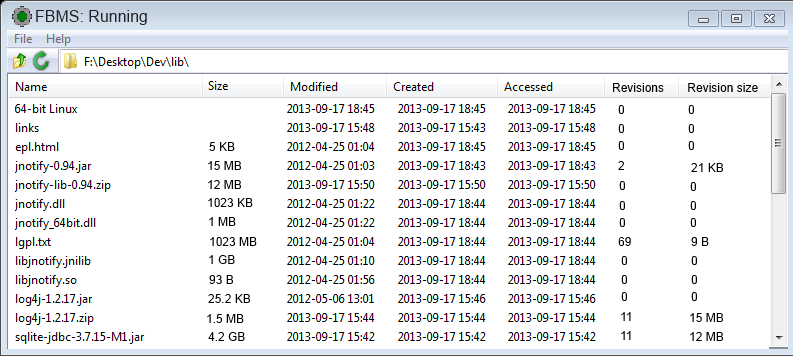
\includegraphics[width=\linewidth]{images/concept.png}

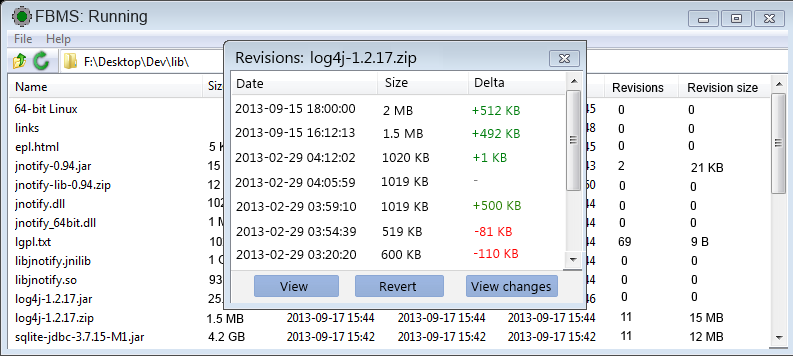
\includegraphics[width=\linewidth]{images/concept2.png}

Our final result is very similar to the mockups:

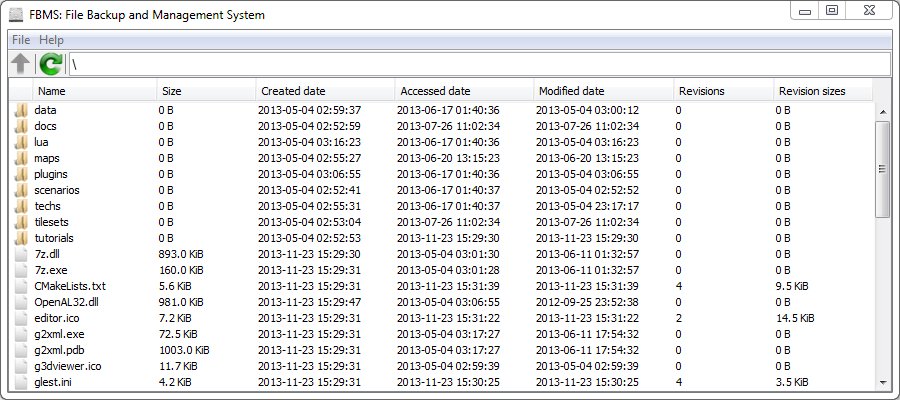
\includegraphics[width=\linewidth]{images/real.png}

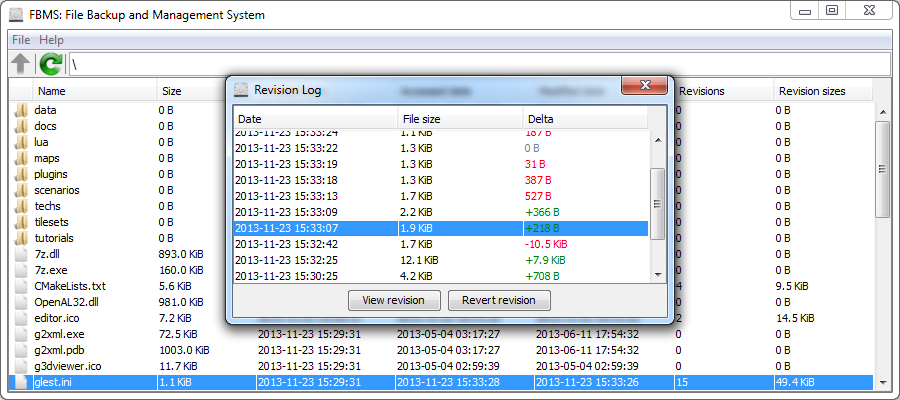
\includegraphics[width=\linewidth]{images/real2.png}

\section{Requirements and early design}

\subsection{Summary use cases}
\subsubsection{List of all use cases}
\begin{itemize}
\item \textbf{Create file}: A file is created. The file will be backed up.
\item \textbf{Modify file}: A file is modified. The file will be backed up and revisioned.
\item \textbf{Rename file}: A file is renamed. Any existing revisions will be renamed to the new name.
\item \textbf{Delete file}: A file is deleted. No other operations will be done on that file.
\item \textbf{Create folder}: A folder is created. Empty folders are not backed up. Folders are created automatically when files are backed up.
\item \textbf{Rename folder}: A folder is renamed. Any existing revisions containing this folder in their path will be renamed to the new name.
\item \textbf{Delete folder}: A folder is deleted. No other operations will be done on that folder.
\item \textbf{Startup}: The program is started up. The location of the backup directory will be determined, database connection established, startup scan commenced, and file watcher initialized. If necessary, first run wizard will be run.
\item \textbf{First run setup}: First run wizard is run if the program determines this is the first run (or regular startup cannot be commenced). Gets from the user the locations of the backup and live directories.
\item \textbf{Change live directory}: The live directory is changed to a new, user specified location. The directory's files are scanned for differences from the backup and the watcher is reinitialized.
\item \textbf{Change backup directory}: The backup directory is changed to a new, user specified location. The previous backup directory's contents are copied to the new location.
\item \textbf{Change settings}: A settings window displays available settings. On close, the settings are saved.
\item \textbf{View backed up files}: The main window is opened by double clicking the system tray icon. The window lists the contents of the backup directory, including files that were deleted or renamed in the live directory.
\item \textbf{Go into folder}: A folder in the main window's file browser is double clicked. The main window's contents are replaced with the contents of that directory (in other words, the contents of a different directory are displayed).
\item \textbf{Go up a directory}: The up button in the main window is clicked. The main window's contents are replaced with the contents of the directory "up" from the current folder. Cannot go up further than the backup directory.
\item \textbf{Refresh the current directory}: The refresh button in the main window is clicked. The main window's contents are replaced with the contents of the current directory. This allows the user to see any updates to the contents of the directory.
\item \textbf{Navigate to a user specified directory}: The file browser location bar is changed and the user presses enter. The entered path is parsed and navigated to as though the user went into that folder. If the path is invalid, the user is alerted.
\item \textbf{View list of revisions for a file}: A file is double clicked in the main window's file browser. A modal displays all available revisions. The time stamp, file size, and difference in file size is shown.
\item \textbf{View revision}: In the revisions dialog, the user double clicks on a revision or selects a revision and clicks the ``view revision'' button. The revision is obtained and opens in the user's default program for that file type.
\item \textbf{Revert revision}: In the revisions dialog, the user double clicks on a revision or selects a revision and clicks the ``view revision'' button. The revision is obtained and is copied to the live directory. A revision is created for the revert operation.
\end{itemize}

\subsubsection{Create file} 
\begin{description}
	\item \textbf{Level}  \\
	Summary
	\item \textbf{Actors} \\
	System
	\item \textbf{Goal} \\
	Add the file created by user to the system and backup it.
	\item \textbf{Activities} \\
	The system receives a file created notice from the watcher module, and put it in file created list.\\
	The file change handler will process the list:
	\begin{enumerate}
		\item[a)]A file with the same name and location exists in the system: \\
		The system will treat the file as a modified file, and make a diff  file for it.
		\item[b)]No file with the same name and location exists in the system: \\
		The system just simply copies the file into the backup folder. Then a new record will be added in database stating a new file added.
	\end{enumerate}
	\item \textbf{Quality} \\
	This is a main use case in the system and must work to a very high standard.
	\item \textbf{Version} \\
	26 November 2013	
\end{description}

\subsubsection{Modify file}
\begin{description}
	\item \textbf{Level} \\
	Summary
	\item \textbf{Actors} \\
	User
	\item \textbf{Goal} \\
	Backup the modified file and make a revision for the change.
	\item \textbf{Activities} \\
	The watcher module notices the file has been modified and adds it to the modified files list. The file change handler for modified files will then handle the files in this list, making a revision for the changes and then copying the file to the correct folder in the backup directory.
	\item \textbf{Quality} \\
	This is a main use case in the system and must work to a very high standard.
	\item \textbf{Version} \\
	27 November 2013	
\end{description}

\subsubsection{Rename file}
\begin{description}
	\item \textbf{Level} \\
	Summary
	\item \textbf{Actors} \\
	System
	\item \textbf{Goal} \\
	Reflect the effect of renaming a file.
	\item \textbf{Activities} \\
	The system receives a file renamed notice from the watcher module, and put it in file renamed list.\\
	The file change handler will process the list: \\
	The system will either make a diff file or copy the file to backup folder.
	\item \textbf{Quality} \\
	This is a main use case in the system and must work to a very high standard.
	\item \textbf{Version} \\
	26 November 2013	
\end{description}

\subsubsection{Rename folder}
\begin{description}
	\item \textbf{Level} \\
	Summary
	\item \textbf{Actors} \\
	User
	\item \textbf{Goal} \\
	When a folder is renamed, ensure that the revisions have the corrected path.
	\item \textbf{Activities} \\
	The watcher notices the folder has been renamed and adds it to the renamed list. The file change handler for renamed files will later handle the paths in this list, copying the folder in the backup directory to the new name and renaming revisions in the database to the new path.
	\item \textbf{Quality} \\
	This is a main use case in the system and must work to a very high standard.
	\item \textbf{Version} \\
	27 November 2013
\end{description}

\subsubsection{Delete file}
\begin{description}
	\item \textbf{Level} \\
	Summary
	\item \textbf{Actors} \\
	System
	\item \textbf{Goal} \\
	Allows the user to delete a specified file 
	\item \textbf{Activities} \\
	User scrolls over live directory and finds the file to be deleted. JNotify notices the file change and calls the watcher. The watcher notices a file has been deleted from the live directory and add to the list. The control reads the list and removes any other instances of the file in the other list. 
	\item \textbf{Quality} \\
	This is a main use case in the system and must work to a very high standard.
	\item \textbf{Version} \\
	28 November 2013
\end{description}

\subsubsection{Revert Revision} 
\begin{description}
	\item \textbf{Level}  \\
	Summary
	\item \textbf{Actors} \\
	User
	\item \textbf{Goal} \\
	Ability to revert a file to a prior version.
	\item \textbf{Activities} \\
	The file selects a revision using the GUI. Backend then uses FileHistory and FileOp to revert the file in such a way as not to interfere with versioning. 
	\item \textbf{Quality} \\
	This part of the program is high priority, it is not critical to the backup functionality of the program but is necessary for the user to take advantage of the versioning information being created.
	 To that end it is also a primary component to why a user would use our program. 
	\item \textbf{Version} \\
	26 November 2013	
\end{description}

\subsubsection{View revision}
\begin{description}
	\item \textbf{Level}  \\
	Summary
	\item \textbf{Actors} \\
	User
	\item \textbf{Goal} \\
	Ability to revert a file to a prior version.
	\item \textbf{Activities} \\
	The user selects whatever file he/she wants to view a specific revision for that file. With a selected file, the user is presented a list of revisions and options, which include view revision. 
	\item \textbf{Quality} \\
	This is a main use case in the system and must work to a very high standard. 
	\item \textbf{Version} \\
	26 November 2013	
\end{description}

\subsubsection{First run setup}
\begin{description}
	\item \textbf{Level}  \\
	Summary
	\item \textbf{Actors} \\
	User
	\item \textbf{Goal} \\
	To setup the live and backup directories on the first time the program is run 
	\item \textbf{Activities} \\
	The program determines if it is the first run by checking for the existence of the file which specifies the backup directory. If this 	file is not found or the backup directory is invalid, it is considered to be the first run. A GUI wizard is shown, and the user is 			asked if they wish to specify a new backup or if they wish to import an old backup. To create a new backup, the user is 				prompted for paths for a live and backup directory (which cannot be children of one or the other). To import an old backup, the 	user is prompted to provide a path to the backup folder (which contains a database file). If the user enters invalid paths, they 		will be prompted to enter a new one. The wizard also allows the user to go back and change previously made choices. On the 			final screen of the wizard, the program initializes the backup and live directories and creates the database connection. 
	\item \textbf{Quality} \\
	This aspect of the program is top priority, as it is mandatory for the program to be used at all. Therefore, it must be completely 	stable and well designed. In fact, this portion of the program is already complete in our prototype, as will be demonstrated in 			section 9. 
	\item \textbf{Version} \\
	28 November 2013	
\end{description}

\subsubsection{Change live directory}
\begin{description}
	\item \textbf{Level} \\
	Summary
	\item \textbf{Actors} \\
	User
	\item \textbf{Goal} \\
	Change the folder system monitors.
	\item \textbf{Activities} \\
	User select "Change live directory" in main window.\\
	The system changes configuration in database, removes the old watcher and adds a new watcher for new live folder.\\
	\item \textbf{Quality} \\
	This is a median use case in the system and should work to a high standard.
	\item \textbf{Version} \\
	26 November 2013	
\end{description}

\subsubsection{Change backup directory}
\begin{description}
	\item \textbf{Level} \\
	Summary
	\item \textbf{Actors} \\
	User
	\item \textbf{Goal} \\
	Change the folder for storing backups.
	\item \textbf{Activities} \\
	User select "Change backup directory" in main window.\\
	The system changes configuration in database, and copies the old folder and its content to the new location.\\
	The old backup folder still lives.
	\item \textbf{Quality} \\
	This is a median use case in the system and should work to a high standard.
	\item \textbf{Version} \\
	26 November 2013
\end{description}

\subsection{Fully-dressed use cases}
\subsubsection{Create File}
\begin{description}
	\item \textbf{Scope} \\
		FBMS
	\item \textbf{Level} \\
		User goal
	\item \textbf{Primary actor} \\
		Main system
	\item \textbf{Stakeholders and interests} \\
		User: Want this new created file is automatically backed up.
	\item \textbf{Preconditions} \\
		The Watcher module is running normally.\\
		There is enough space in backup folder.\\
		System has read access to the newly created file.
		System has write access to backup folder.
	\item \textbf{Success Guarantee} \\
		The newly created file is backed up.\\
		Records are added in database.\\
		The history of this file is accessible from GUI.
	\item \textbf{Main Success scenario} \vspace{-4ex} \\
	\begin{itemize}
		\item[(1)] The system received a file created notice, and put it in file created list.
		\item[(2)] The system determines whether a file with the same name and location has been existed in the backup folder.
		\item[(3a)] If so, the system treated this file as a modified file.\\
					Remove this file form file create list. Add it to file modified list.\\
					Make a diff file for this file.
		\item[(3b)] If not, copy this file to backup folder.
		\item[(4)] Add a record in database.
	\end{itemize}
	\item \textbf{Extensions} \\
		The file will be locked when being copied to backup folder.
	\item \textbf{Special Requirements}\\
		Privilege is possible required.
	\item \textbf{Technology and Data Variations List}\\
		The program flow changes based on whether a file with the same name and location has been existed in the system. If it exists, system will do additional steps to ensure no wrong overwriting occurs. If not, system will do it in regular way.
	\item \textbf{Frequency of Occurrence}\\
		Every time a new file is created in live folder.
\end{description}

\subsubsection{First Run}
\begin{description}
	\item \textbf{Scope} \\
		Program is run for the first time 
	\item \textbf{Level} \\
		User goal
	\item \textbf{Primary actor} \\
		User 
	\item \textbf{Stakeholders and interests} \\
		User: Setup the program with the directories it will act on.
	\item \textbf{Preconditions} \\
		It is the program's first run or the program cannot startup normally. 
	\item \textbf{Success Guarantee} \\
		The backup and live directories are configured to valid paths.
	\item \textbf{Main Success scenario} \vspace{-4ex} \\
	\begin{itemize}
		\item Program determines that it is the first run because the file pointing to the backup location is missing, or the backup location is otherwise invalid (non-existent folder or missing necessary database file inside this folder). 
		\item A GUI wizard is displayed, with buttons for navigating and exiting the wizard. 
		\item The wizard prompts the user as to whether they wish to create a new backup or import an existing backup. 
				If a new backup is chosen, the user is prompted to provide paths for both the live and backup directories (via file choosers). 
				If the user chooses to import an existing backup, they are prompted to provide a path to this backup directory. 
		\item The wizard finalizes, telling the user that setup was completed. 
		\item The program establishes a connection with the database, setting it up in the specified backup directory by creating the file that points to the backup directory. 
	\end{itemize}
	\item \textbf{Extensions} \\
	\begin{itemize}
		\item The user cannot specify live and backup directories that are children or parents of each other. 
				This prevents infinite recursion. If the backup folder was inside the live directory, every backup would be identified as a change to the live directory (and thus need to be backed up as well). If the live directory was inside the backup directory, then we 					run the risk of backed up files overwriting files in the live directory. 
				The program will issue an error dialog if this occurs, and will not allow the user to continue until they specify valid directories. 
		\item When importing an existing backup, the chosen directory must contain a database file which indicates that the directory has been used for backup before. 
				This file contains the path of the live directory, which is necessary for the program to import an existing backup. 
				The program will issue an error dialog if this occurs, and will not allow the user to continue until they specify a valid directory. 
				If the user closes the dialog window, it will do nothing unless they are on the final panel of the wizard, which indicates a success. 
	\end{itemize}
	\item \textbf{Special Requirements}\\
		The program directory and the chosen live and backup directories must have write access.
	\item \textbf{Technology and Data Variations List}\\
		The program flow changes based on whether the user chose to import an existing backup or start a new one. If they chose to import an existing backup, the live directory is set when the program initializes the database. If they started a new backup, the wizard sets 		the live directory.
	\item \textbf{Frequency of Occurrence}\\
		Exactly once when the program starts for the first time 
		May also occur if an error is encountered when the program starts up (such as if the backup directory is invalid) 
\end{description}

\subsubsection{Delete file}
\begin{description}
	\item \textbf{Scope} \\
		FBMS
	\item \textbf{Level} \\
		User goal
	\item \textbf{Primary actor} \\
		User 
	\item \textbf{Stakeholders and interests} \\
		System: don't try and backup a deleted file
	\item \textbf{Preconditions} \\
		A file or folder is deleted
	\item \textbf{Success Guarantee} \\
		The deleted path will be removed from all other file handler lists
	\item \textbf{Main Success scenario} \vspace{-4ex} \\
	\begin{itemize}
		\item A file or folder is deleted by the user.
		\item The watcher detects the deletion and adds it to the list of deleted files. 
		\item The file change handler for deleted files fires before the other file change handlers.
		\item The handler removes the paths in the deleted files list from all the file change lists. This ensures that the other handlers won't try to act on deleted files.
	\end{itemize}
	\item \textbf{Extensions} \\
		None
	\item \textbf{Special Requirements}\\
		None
	\item \textbf{Technology and Data Variations List}\\
		None
	\item \textbf{Frequency of Occurrence}\\
		Once for each deleted file
\end{description}

\subsubsection{Revert file to revision}
\begin{description}
	\item \textbf{Scope} \\
		FBMS
	\item \textbf{Level} \\
		User goal
	\item \textbf{Primary actor} \\
		User 
	\item \textbf{Stakeholders and interests} \\
		User: Revert the selected file to the selected version. 
	\item \textbf{Preconditions} \\
		\begin{itemize}
		\item System must be in a properly setup and running state. 
		\item A file must be selected by the user. 
		\item The file must be within the folder listing that is currently being backed up. .
		\item A version must be selected by the user. 
		\item A version history must exist for the file. 
		\item System has proper read/write access to the backup and the system file. 
		\end{itemize}
	\item \textbf{Success Guarantee} \\
		\begin{itemize}
		\item The selected file is reverted to the proper revision. 
		\item The previous version that was overwritten still remains in backup as a version. 
		\end{itemize}
	\item \textbf{Main Success scenario} \vspace{-4ex} \\
	\begin{itemize}
		\item User prompts the program via the GUI that they wish to make a file revision. 
		\item The user selects the file in question and then selects the revision they desire from the selection. 
		\item The system then goes through file history to find the proper diff file referenced by the database. 
		\item Temporary files are made where appropriate.
		\item The diff file is used to create a reverted version of the specified file. 
		\item The file specified is now reverted and in the proper location. 
	\end{itemize}
	\item \textbf{Extensions} \\
		\begin{itemize}
		\item Only files within the specified backup environment will have versions stored to revert to. 
		\item Nothing will happen if the user selects the file and revision and exits the dialogue or otherwise does not hit ‘Ok’.  
		\item If the function fails due to system level issues, like permission conflicts, the function ends and the user is notified.  
	\end{itemize}
	\item \textbf{Special Requirements}\\
		Require write/read access to the file being modified. 
	\item \textbf{Technology and Data Variations List}\\
		None
	\item \textbf{Frequency of Occurrence}\\
		Whenever specified by the user.
\end{description}

\subsubsection{Rename file}
\begin{description}
	\item \textbf{Scope} \\
		FBMS
	\item \textbf{Level} \\
		User goal
	\item \textbf{Primary actor} \\
		User 
	\item \textbf{Stakeholders and interests} \\
		User: Want this renamed file is automatically renamed in system. 
	\item \textbf{Preconditions} \\
		\begin{itemize}
		\item The Watcher module is running normally. 
		\item The reversion is accessible. 
		\item System has read access to the newly created file. 
		\item System has write access to backup folder.   
		\end{itemize}
	\item \textbf{Success Guarantee} \\
		\begin{itemize}
		\item The backups of file renamed are renamed. 
		\item Records are renamed in database. 
		\end{itemize}
	\item \textbf{Main Success scenario} \vspace{-4ex} \\
	\begin{itemize}
		\item System is notified for the renaming operation. 
		\item System renames all the backups of the file.  
		\item System add a rename record into the database.  
		\item System changes all the records of the file. 
	\end{itemize}
	\item \textbf{Extensions} \\
		\begin{itemize}
		\item The backups of file will be locked when being renamed.     
	\end{itemize}
	\item \textbf{Special Requirements}\\
		None 
	\item \textbf{Technology and Data Variations List}\\
		None
	\item \textbf{Frequency of Occurrence}\\
		Every time a file is renamed in live folder.
\end{description}

\subsection{Use case diagram}
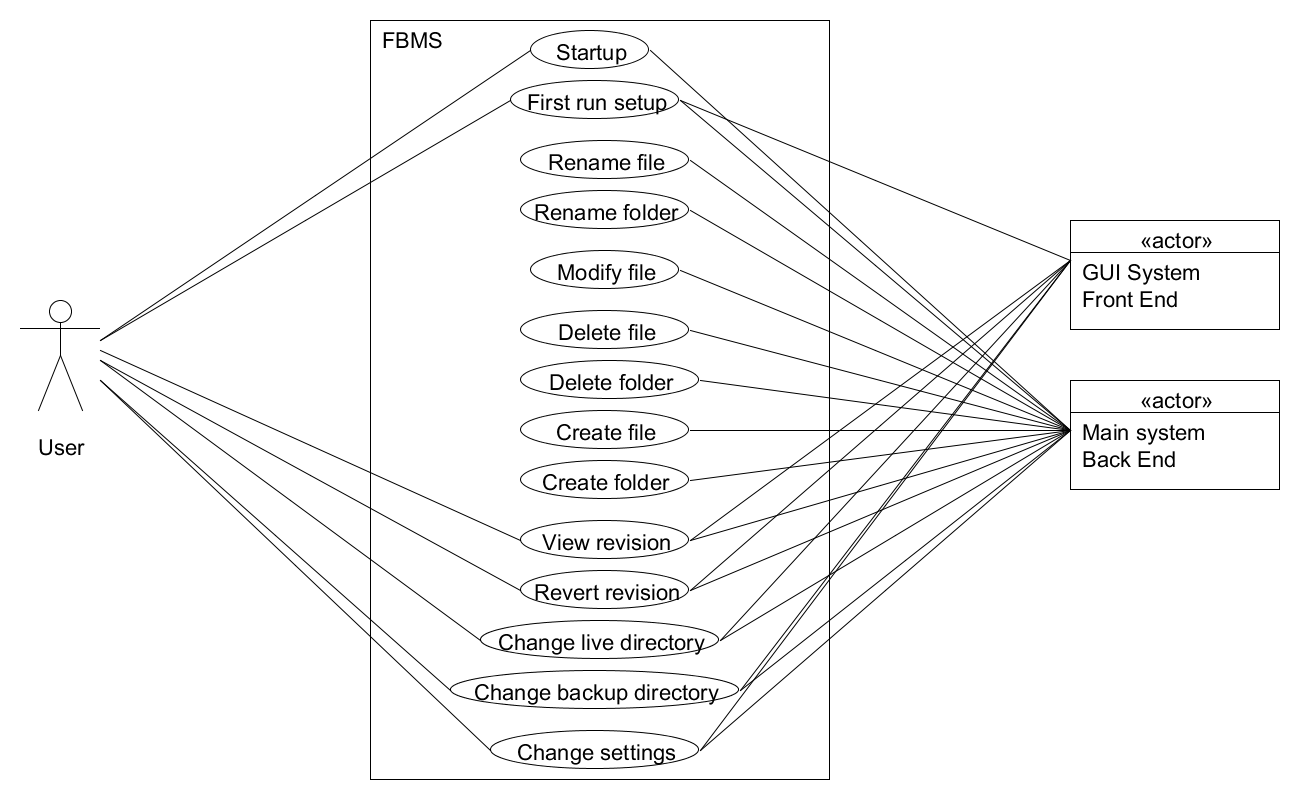
\includegraphics[width=\linewidth]{images/use_cases.png}

\subsection{Domain model}
\todonote{Butler. Make from scratch.}

\subsection{Glossary}
\begin{itemize}
\item \textbf{Live directory}: The directory that the program monitors for changes. In other words, the directory that is being backed up.
\item \textbf{Backup directory}: The directory where the backed up files and revisions from the live directory are placed.
\item \textbf{Revision}: A snapshot of a file at a given time.
\item \textbf{Patch}: Data that details what changed from one revision of a file to another. Also called a ``diff''.
\item \textbf{Raw data}: The contents of a file as bytes, without any kind of interpretation.
\item \textbf{Revision database}: The database where revisions are stored as patch files (for plain text) or raw data (for binary).
\item \textbf{File operations}: Operations that change a file's content, name, or location. This includes operations such as file creation, renaming, moving, or deletion.
\item \textbf{Error alerts}: GUI dialogs that alert the user to an error. They are split into two branches:
	\begin{itemize}
	\item \textbf{Fatal alerts}: Obtrusive dialogs that indicate that the program cannot proceed.
	\item \textbf{Non-fatal alerts}: Non-obtrusive dialogs that appear in the bottom right corner of the screen and automatically disappear after some time. These indicate something has gone wrong and cannot be recovered, but do not halt the progress of the program. For example, a file that cannot be backed up (perhaps due to permission issues).
	\end{itemize}
\item \textbf{Front end}: The visible portions of the program, including the main GUI window, the toolbar icon, and dialogs.
	\begin{itemize}
	\item \textbf{Main frame}: The large window that is opened by double clicking the program's system tray icon. It lists the files and folders inside the backup directory and offers actions on these files.
	\item \textbf{Revisions dialog}: The modal opened by double clicking on a file in the main frame's list of files. It displays a list of revisions for that file, and offers actions on these revisions.
	\item \textbf{Settings dialog}: The modal opened by from the ``settings'' option in the main frame's menus. It offers customization of some features such as trim, whether or not to perform the startup scan, and the display of errors.
	\end{itemize}
\item \textbf{Watcher}: The program component that watches the live directory for changes. It operates concurrently from the rest of the program.
\item \textbf{File change handlers}: The section of the program that handles changes in files (file operations). Runs concurrently from the rest of the program.
\item \textbf{Data retriever}: The program component that fetches data about revisions or the file system for the front end.
\item \textbf{First start wizard}: A wizard that is shown on the first start (or if normal startup cannot occur). It guides the user in choosing the live and backup directories.
\item \textbf{Trim}: A program feature that removes revisions older than a configured date.
\item \textbf{Startup scan}: The one-time scan that occurs when starting the program up (or after the live directory is changed). This allows the backup of files that were changes when the system was not running, but is an unnecessary overhead if the system is always running. Can be disabled in the settings dialog.
\end{itemize}

\subsection{Supplementary specification}
\subsubsection{Vision}
FBMS is a multiplatform, self-contained automated backup and revision program. It does not require cloud services or any online access to function. It uses local resources and ideally secondary drive locations to backup critical data.

We chose this project as it fills a gap between cloud backup platforms and weighty software suites requiring considerable infrastructure and resources. Our program takes advantage of external drives or mapped network drives and consolidates folders specified by the user to a secure location. Joined with a redundant hardware solution like RAID, our software is a suitable replacement to cloud services.

Our design choices have lead to a cross platform utility that should be usable on any operating system supported by the Java run time. This frees it from the majority of dependencies that weigh down other software.

Using the data we backup we are able to run and operate a versioning system. This allows a user to revert unwanted file changes, restore corrupted files, or replace files accidentally deleted. It takes a step further then previous versions in windows, or other similar systems like svn. This gives more control over where versions are kept and is more straightforward then other versioning systems. 

\subsubsection{Interfaces}
The interface consists of the GUI windowing system along with a minimizer tray icon. Closing the GUI minimizes the application to an icon in the system tray. This means that the application does not end simply by pressing the “x” button on the GUI but needs to be shut down from the system tray icon which has an “exit” option for closing the application entirely. We have tried to make the main GUI as simple as possible so that an average user could be able to handle the software. It comprises of a few simple areas namely a table, a toolbar, and a menubar. 

\textbf{Table}: This is used to display the contents of the backup directory. This directory is specified by the user and shows detailed entries of the names of the files or the folder, the sizes, the modified and the created dates as well as the last date it was accessed on and finally the revision size and the number of current revisions. Interactive features of the table include a scrollbar, which the user can use to scroll up and down the list and selection, allowing the user to select a single file at a time. 
When a folder is selected the table refreshes the contents of the list by generating the contents of the folder. Selecting a file opens up a dialog box with information of the file revisions. Errors are handled by the means of dialog boxes. 

\textbf{Toolbar}: This is located above the table and contains two buttons and a text field. One of the button is an up button enabling the user to navigate out of the current folder. However the button is disabled if the user is already in the backup directory. The second button is the refresh button which refreshes the directory to the latest version. The text field is set to contain the current path of the directory and is also disabled if the user is already in the back up directory. 

\textbf{Menubar}: At the very top is a menubar which consists of a file and a help item. The file item expands to options of: 

\begin{itemize}
\item \textbf{View revisions}: It works in the same was a double clicking a file (eg, opens the revision dialog box; if no files are selected, do nothing). The dialog has options of view and revert which enables the user to view the revision of the file selected. This gives the information in the form of a JTable which shows the name of the file, its size and the modified size in bytes. The revert reversion removes any changes and changes to the file to the original state.
\item \textbf{Copy-to}: Creates a dialog for selecting the folder to copy the selected file to. Like review revisions, this cannot be done if no file is selected. 
Restore all: Prompts the user (with a dialog box) if they're sure they want to continue. Upon approval, the directory is restored to the previous revision. 
Settings\item \textbf{Settings}: This has a number of interesting options like removing revisions older than a particular number of days, which the user can specify in a text box, and controlling the sizes of the files set for revision.  Furthermore, a user can also enable or disable the scanning of the directories at start-up by the means of a check box. Lastly they can choose whether they want non fatal displayed or not.
\item \textbf{Exit}: Closes the GUI window. However it can be brought back by clicking on the icon in the system tray. 
\item \textbf{Help}:The help menu has a single option to display the online help. This opens the website for the software in the users default browser. 
\end{itemize}

\subsubsection{Reliability}
To maximize efficiency, the watcher module, which notices changes to files, adds these changes to lists. At specific intervals, the program handles the files in these lists. This reduces the program's use of system resources by allowing the program to frequently sleep instead of constantly looping while the program is running. It also drastically reduces the number of file operations. Some operating systems and programs will actually modify a file multiple times in just a few milliseconds (even if the file only appears to have been modified once from the user's perspective). The interval based system combines duplicate operations. So if the user modifies a file a dozen times within the interval, the program only stores one modification as a revision (with that revision being all the changes since the file was last modified).
\\Similarly, we use the JNotify library specifically because it binds with the operating systems for maximum performance. At one early point of time, we actually considered checking all the files in the live directory for changes in their CRC value, which would have been much slower.
\\The program also handles errors in a user-friendly way. Fatal errors are displayed as dialog boxes and also copied to the log (which helps find the source of errors). Non-fatal errors use a non-obtrusive error pop-up message that appears in the bottom corner of the screen and disappears on its own after a few seconds.
Finally, when file operations cannot be performed on a file (for reasons such as the file being open in another program or invalid permissions), the operation is retried after a short delay before informing the user of the error (which is a non-fatal error, as the file can simply be skipped).


\subsubsection{Supportability}
\begin{itemize}
	\item \textbf{OS Compatibility} \\
	To adapt different OSes, we are storing a relative path in database. It solves the problem of changing backup folder.
	\item \textbf{Logging} \\
	Log is provided to diagnose problem when error occurs.\\
	Through analysing the log it is possible to give out a solution.
	\item \textbf{Import from old backup} \\
	It is possible to import backups from an old backup folder.\\
	This function is provided in first run wizard.
	\item \textbf{Configuration} \\
	Live folder and backup folder could be changed.
\end{itemize}

\subsubsection{Third party components}
The project uses third party components for several areas, allowing the project to be completed in a reasonable span of time, as well as assisting in functionality beyond our current skills. Currently, we use:

\begin{itemize}
\item \textbf{JNotify}: This library is used to detect changes in the live directory. It is capable of running event handlers when file changes occur. This allows us to efficiently find the changes in the directory. JNotify binds with the operating system (in which it supports all the major operating systems), allowing it to function similar to an interrupt-style listener. The program will then use a polling system to perform file operations on changes that occurred since the last poll. This makes spotting changes fast while minimizing file operations (which often occur in multiples even if the operation appeared atomic to the user).
\item \textbf{Log4j}: The well known logging library is used to making logging efficient and configurable. Most importantly, it allows us to set levels to our logging. When the logging is set to DEBUG, the logging system is very verbose. This is useful when we need to know exactly what the program is doing, but for general usage, this slows the program down and floods the logs with irrelevant information. Normally, the user will have the logging set to either WARN or ERROR, which will limit the logging to things that are of actual use to the user.
\item \textbf{Diff match patch}: This library is used to generate patch files, which is what our revisioning system is based on. The library is also used to apply the patches, restoring the originals. To restore files several revisions old, the patch files are daisy-chained, restoring revisions until we get to the one we want.
\item \textbf{SQLite}: We use the SQLite JDBC driver to allow our databases to be well organized into an efficient, minimal file.
\item \textbf{Java MIME Magic}: This library is used to maximize our ability to detect the difference between binary and text files (since they are revisioned differently).
\end{itemize}

We originally planned to use Java-diff-utils as the patching engine, but the library appears to be either bugged or the documentation is incorrect. We switched to the diff match patch library instead, which performed all the functionality we need and was better documented.

These components integrate with our program and were chosen with efficiency in mind.

\subsection{System sequence diagrams}

\subsubsection{First run setup}
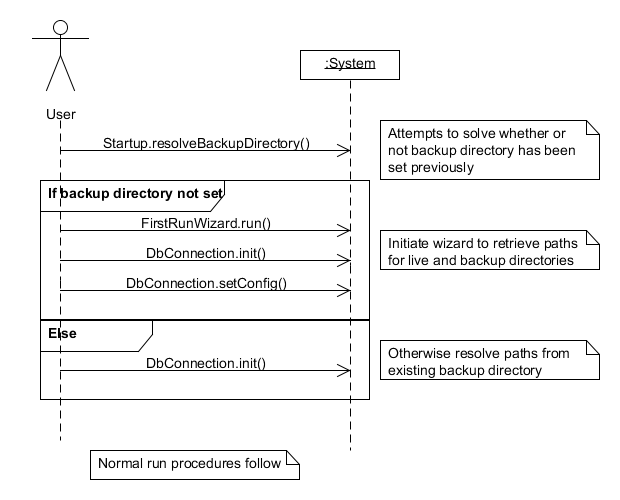
\includegraphics[width=\linewidth]{images/sequence_diagram_first_run.png}

\subsubsection{Revert to file revision}
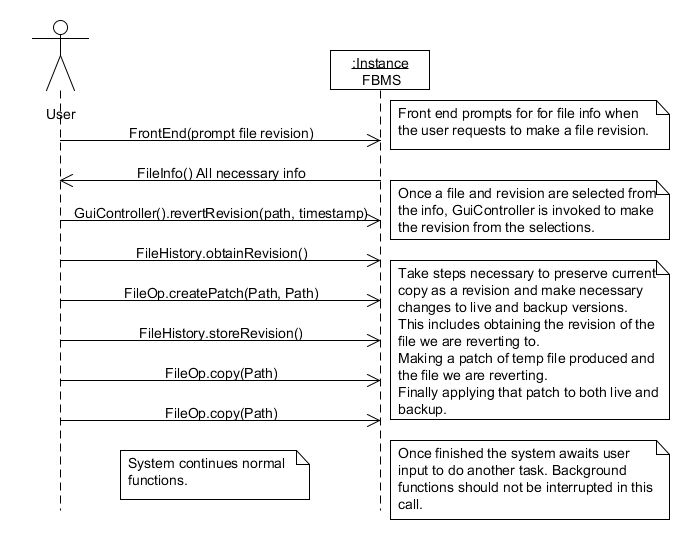
\includegraphics[width=\linewidth] {images/revertRevision_ssd.png}

\subsubsection{Delete file}
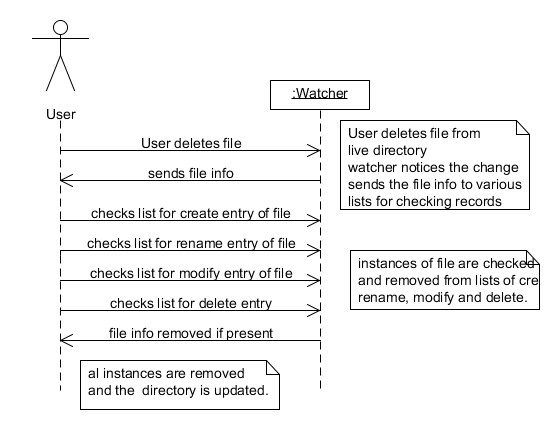
\includegraphics[width=\linewidth]{images/DeleteFileSD.png}

\subsubsection{Rename folder}
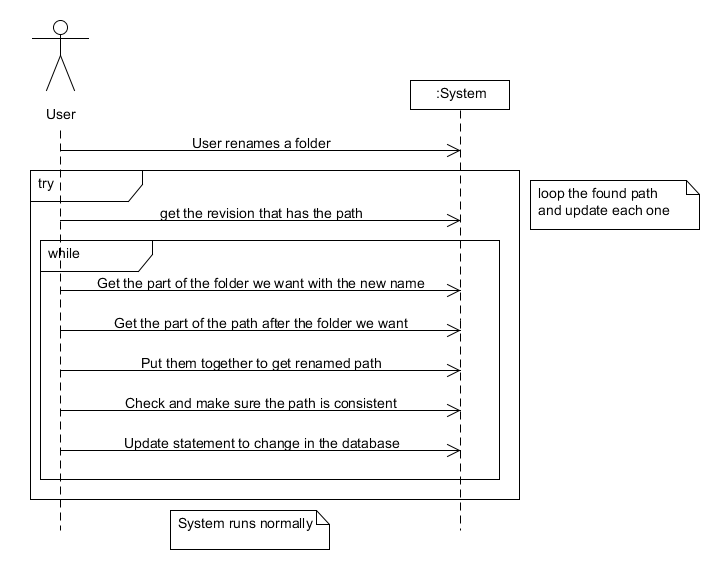
\includegraphics[width=\linewidth]{images/renamefoldersd.png}

\subsubsection{Rename file}
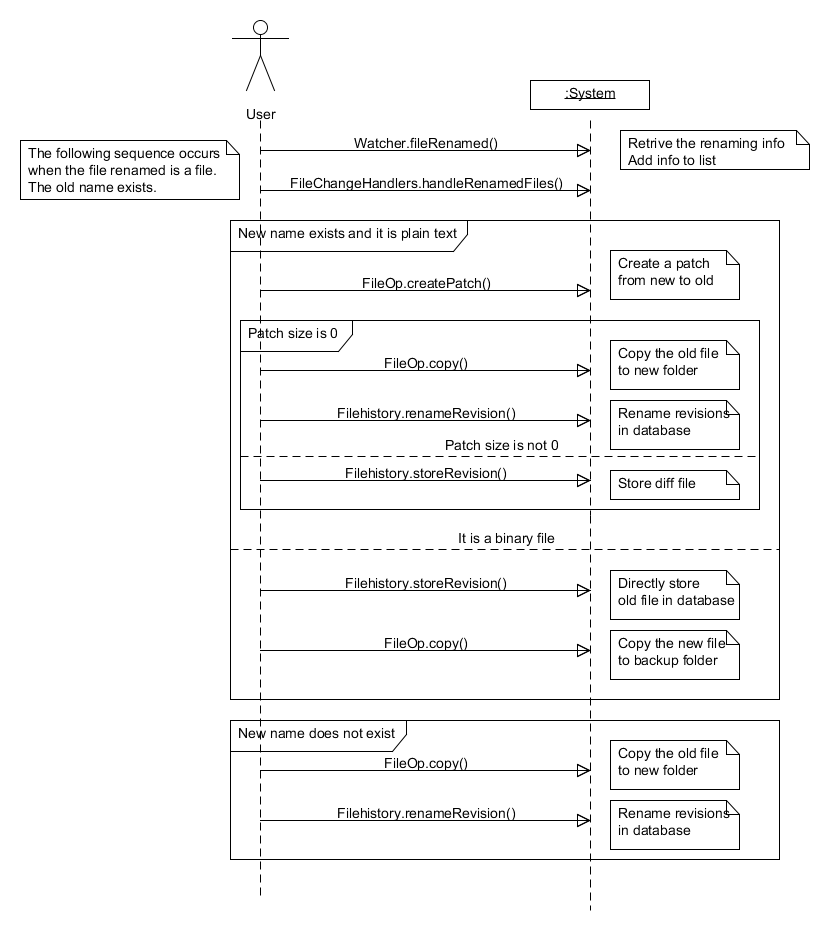
\includegraphics[width=\linewidth]{images/fileRenamed_file_ssd.png}
\newpage
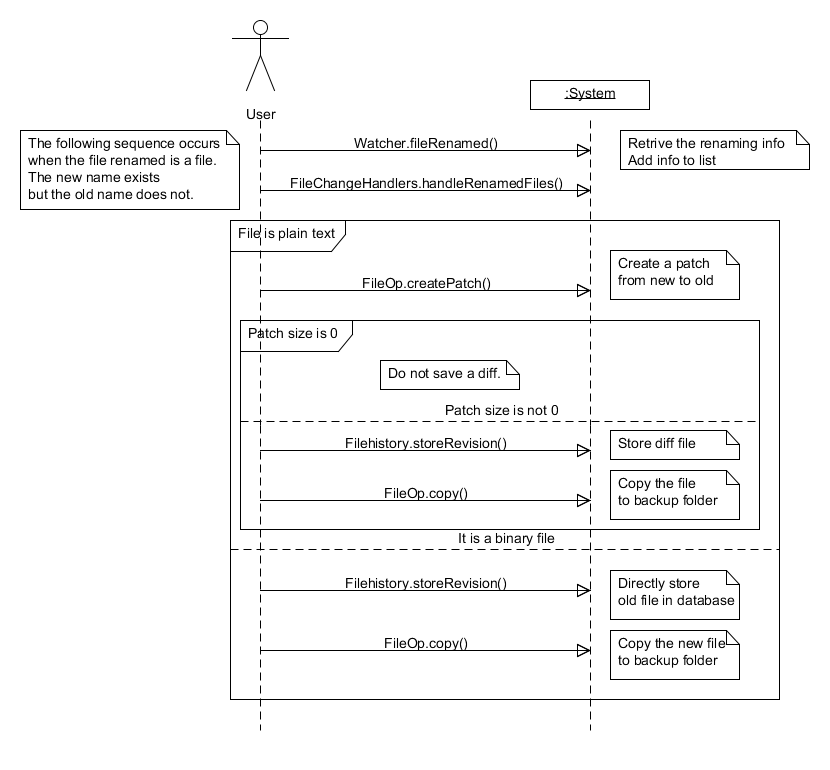
\includegraphics[width=\linewidth]{images/fileRenamed_file2_ssd.png}
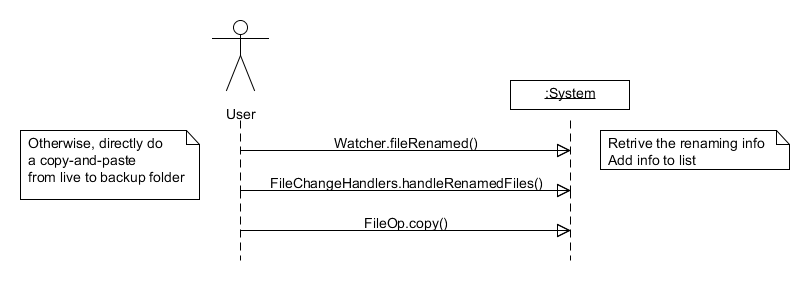
\includegraphics[width=\linewidth]{images/fileRenamed_file3_ssd.png}


\subsection{Operation contracts}
%% This section is a bit messy due to the complex formatting. In particular, we
%% need to manually add line breaks to some of the cross references, which are too
%% long to wrap
\textbf{\texttt{FileOp.createPatch(Path oldRevision, Path currentRevision)}}
\begin{description} 
	\item[Cross references:] \hfill \vspace{-4ex} \\
		\begin{description}
		\item[Operation contracts:] \hfill \\
			\texttt{FileChangeHandlers.handleModifiedFiles()},\\
			\texttt{FileChangeHandlers.handleRenamedFiles()},\\
			\texttt{Startup.startupScan()}
		\item[Use cases:] \hfill \\
			\texttt{Startup}, \texttt{Rename file}, \texttt{Modify file},\\
			\texttt{View revision}, \texttt{Revert revision}
		\end{description}
	\item[Precondition:] \texttt{oldRevision} and \texttt{currentRevision} exist
	\item[Postconditions:] A \texttt{Path} is created. It points to a temporary file containing the patch to patch \texttt{currentRevision} to \texttt{oldRevision}.
\end{description}

\vspace{0.75cm}

\textbf{\texttt{FileOp.applyPatch(Path currentRevision, Path patchFile)}}
\begin{description}
	\item[Cross references:] \hfill \vspace{-4ex} \\
	\begin{description}
		\item[Operation contracts:] \hfill \\
			\texttt{FileHistory.displayRevision(Path, long)}
		\item[Use cases:] \hfill \\
			\texttt{View revision}, \texttt{Revert revision}
	\end{description}
	\item[Precondition:] \texttt{currentRevision} and \texttt{patchFile} exist
	\item[Postconditions:] Creates a temporary file, which contains the contents of the 		\texttt{currentRevision} with \texttt{patchFile} applied to it.
\end{description}

\vspace{0.75cm}

\textbf{\texttt{DataRetriever.getFolderContents(Path folder)}}
\begin{description}
	\item[Cross references:] \hfill \vspace{-4ex}  \\
	\begin{description} 
		\item[Operation contracts:] \hfill \\
			\texttt{Data.getTableData(Path)}
		\item[Use cases:] \hfill \\
			None
	\end{description}
	\item[Precondition:] Path \texttt{folder} exists
	\item[Postconditions:] A \texttt{List<FileInfo>} is returned, containing the content of the \texttt{folder}
\end{description}

\vspace{0.75cm}

\textbf{\texttt{GuiController.displayRevision(Path file, long timestamp)}}
\begin{description}
	\item[Cross references:] \hfill \vspace{-4ex}  \\
	\begin{description} 
		\item[Operation contracts:] \hfill \\
			\texttt{RevisionTableSelectionListener.activateRow()}
		\item[Use cases:] \hfill \\
			\texttt{View revision}
	\end{description}	
	\item[Precondition:] A revision exists in the database for the specified file and time stamp
	\item[Postconditions:] A temporary file of the specific revision is created. System will open the file with default application for the file type
\end{description}

\vspace{0.75cm}

\textbf{\texttt{GuiController.changeLiveDirectory(Path newDirectory)}}
\begin{description}
	\item[Cross references:] \hfill \vspace{-4ex}  \\
		\begin{description} 
		\item[Operation contracts:] \hfill \\
			\texttt{MainMenu.initFileActions()}
		\item[Use cases:] \hfill \\
			\texttt{Change live directory}
	\end{description}	
	\item[Precondition:] \texttt{newDirectory} exists and is valid (not a parent or child of backup directory)
	\item[Postconditions:] \texttt{Main.liveDirectory} is changed to \texttt{newDirectory}. The previous file watcher is cancelled. A new file watcher is created for the new live directory. Files in the live directory are scanned once to backup
\end{description}

\vspace{0.75cm}

\textbf{\texttt{Startup.resolveBackupDirectory()}}
\begin{description}
	\item[Cross references:] \hfill \vspace{-4ex}  \\
		\begin{description} 
		\item[Operation contracts:] \hfill \\
			\texttt{Main.main(String[])}
		\item[Use cases:] \hfill \\
			\texttt{Startup}
	\end{description}
	\item[Precondition:] None
	\item[Postconditions:] \texttt{Main.backupDirectory} is set to contents of \texttt{backup\_{}location} file if it exists and is valid. First run will begin if backup directory cannot be resolved
\end{description}

\vspace{0.75cm}

\textbf{\texttt{DbConnection.getFileRevisions(Path file)}}
	\begin{description}
	\item[Cross references:] \hfill \vspace{-4ex}  \\
		\begin{description} 
		\item[Operation contracts:] \hfill \\
			\texttt{DataRetriever.getFolderContents(Path)},\\
			\texttt{DataRetriever.getRevisionInfo(Path)},\\
			\texttt{FileHistory.obtainRevisionContent(Path, long)}
		\item[Use cases:] \hfill \\
			\texttt{View revision}, \texttt{Revert revision}
	\end{description}
	\item[Precondition:] \texttt{file} exists
	\item[Postconditions:] \hfill \\
	A \texttt{List<RevisionInfo>} is returned, containing revision infomation of \texttt{file}.
\end{description}

\vspace{0.75cm}

\textbf{\texttt{DbConnection.setConfig(String settingName, String settingValue)}}
\begin{description}
	\item[Cross references:] \hfill \vspace{-4ex}  \\
		\begin{description} 
		\item[Operation contracts:] \hfill \\
			\texttt{GuiController.changeLiveDirectory(Path)},\\
			\texttt{Startup.startup()}
		\item[Use cases:] \hfill \\
			\texttt{Startup}, \texttt{First run setup}, \texttt{Change live directory}
	\end{description}
	\item[Precondition:] The database exists.
	\item[Postconditions:] The field \texttt{settingName} is set to \texttt{settingValue}
\end{description}

\vspace{0.75cm}

\textbf{\texttt{FileOp.copy(Path file, Path destinationFolder)}}
\begin{description}
	\item[Cross references:] \hfill \vspace{-4ex}  \\
		\begin{description} 
		\item[Operation contracts:] \hfill \\
			\texttt{GuiController.changeBackupDirectory(Path)},\\
			\texttt{GuiController.copyTo(Path, Path)},\\
			\texttt{FileChangeHandlers.handleCreatedFiles()}, \\
			\texttt{FileChangeHandlers.handleModifiedFiles()}, \\
			\texttt{FileChangeHandlers.handleRenamedFiles()},\\
			\texttt{GuiController.restoreBackup(Path)},\\
			\texttt{Startup.startupScan(Path)}
		\item[Use cases:] \hfill \\
			\texttt{Startup}, \texttt{Create file}, \texttt{Rename file},
			\texttt{Modify file}, \texttt{Revert revision},\\
			\texttt{Change backup directory}
	\end{description} 	      
	\item[Precondition:] \texttt{file} exists
	\item[Postconditions:] \texttt{file} will be copied to the \texttt{destinationFolder}. If \texttt{destinationFolder} does not exist, it will be created. Any non-existant parent folders up to \texttt{destinationFolder} will be created.\\
	Any existed file will be overwritten.
\end{description}

\vspace{0.75cm}

\textbf{\texttt{FileHistory.storeRevision(Path file, Path diff, long filesize, long delta)}}
\begin{description}
	\item[Cross references:] \hfill \vspace{-4ex}  \\
		\begin{description} 
		\item[Operation contracts:] \hfill \\
			\texttt{FileChangeHandlers.handleModifiedFiles()},\\
			\texttt{FileChangeHandlers.handleRenamedFiles()},\\
			\texttt{GuiController.revertRevision(Path, long)}
		\item[Use cases:] \hfill \\
			\texttt{Startup}, \texttt{Create file}, \texttt{Rename file},
			\texttt{Modify file}
	\end{description}
	\item[Precondition:] \texttt{file} and \texttt{diff} exist
	\item[Postconditions:] A row is inserted into the database containing information about the revision. In addition to the path of the file, the contents of the diff, the file size, and the delta (change in file size), the time will also be stored.
\end{description}

\subsection{Obtaining user feedback}
Most of our user-feedback stems from heavy testing. We have found several bugs by combining manual testing with logging. Features are also prioritized by user feedback. In version 1.0, for example, we had no support for binary revisions. They were backed up, but not revisioned. This was one of the biggest limitations at the time, and reflected by user feedback. In version 2.0, we introduced support for these binary revisions.

Another area where feedback was crucial was in the GUI development. We had to aim to make the GUI both natural and easy to use. For example, the table rows are activated via double clicking or the enter key. The default behavior of the enter key in a table, however, was to go to the next line, which is counter-intuitive for a file browser, and was overridden.

\section{Updated design and unit testing}

\subsection{System operations}
\begin{itemize}
\item \texttt{Startup.resolveBackupDirectory()}
\item \texttt{DbConnection.insertRevision()}
\item \texttt{DbConnection.getFileRevisions()}
\item \texttt{DbConnection.getSpecificRevision()}
\item \texttt{DbConnection.renameRevisions()}
\item \texttt{DbConnection.setConfig()}
\item \texttt{DbConnection.getConfig()}
\item \texttt{FileOp.createPatch()}
\item \texttt{FileOp.applyPatch()}
\item \texttt{GuiController.revertRevision()}
\item \texttt{GuiController.viewRevision()}
\item \texttt{GuiController.changeLiveDirectory()}
\item \texttt{GuiController.changeBackupDirectory()}
\item \texttt{FileChangeHandlers.handleRenamedFiles()}
\item \texttt{FileChangeHandlers.handleCreatedFiles()}
\item \texttt{FileChangeHandlers.handleModifiedFiles()}
\item \texttt{FileChangeHandlers.handleDeletedFiles()}
\item \texttt{FileHistory.getRevisionInfo()}
\item \texttt{FileHistory.storeRevision()}
\item \texttt{FileHistory.obtainRevision()}
\item \texttt{FileHistory.renameRevision()}
\end{itemize}

\subsection{Sequence or communication diagrams with GRASP patterns}
\subsubsection{GuiController.revertRevision}
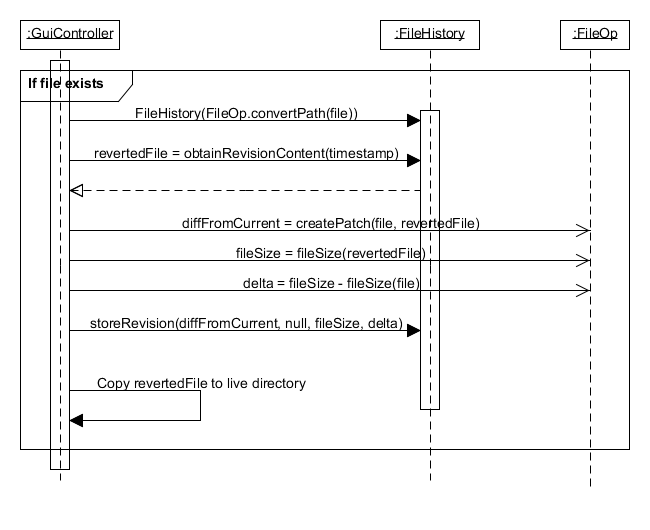
\includegraphics[width=\textwidth]{images/revert_revision_sequence.png}

\subsubsection{GuiController.displayRevision}
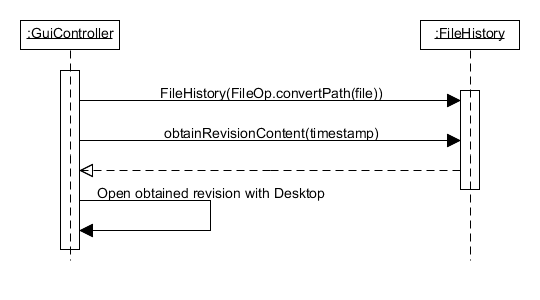
\includegraphics[width=\textwidth]{images/view_revision_sequence.png}

\subsubsection{GuiController.changeLiveDirectory}
\todonote{Butler}

\subsubsection{GuiController.changeBackupDirectory}
\todonote{Butler}

\subsubsection{FileOp.applyPatch}
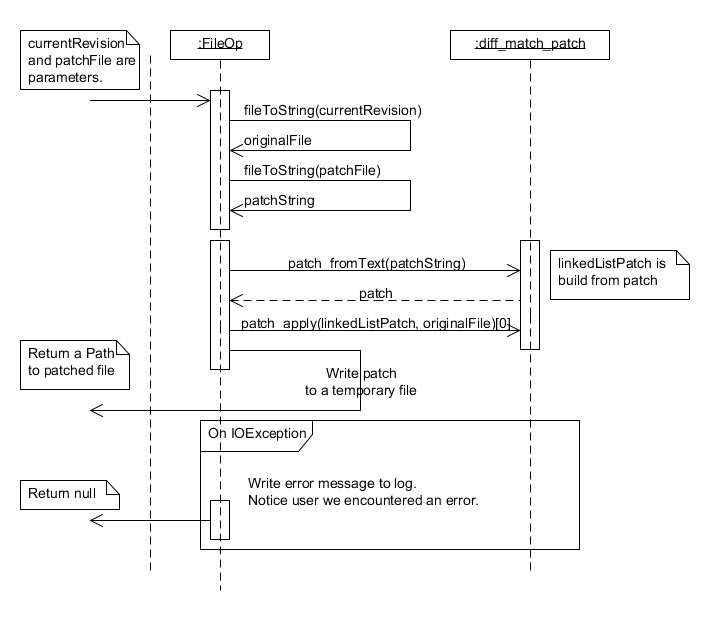
\includegraphics[width=\textwidth]{images/applyPatch_sequence.png}

\subsubsection{FileOp.createPatch}
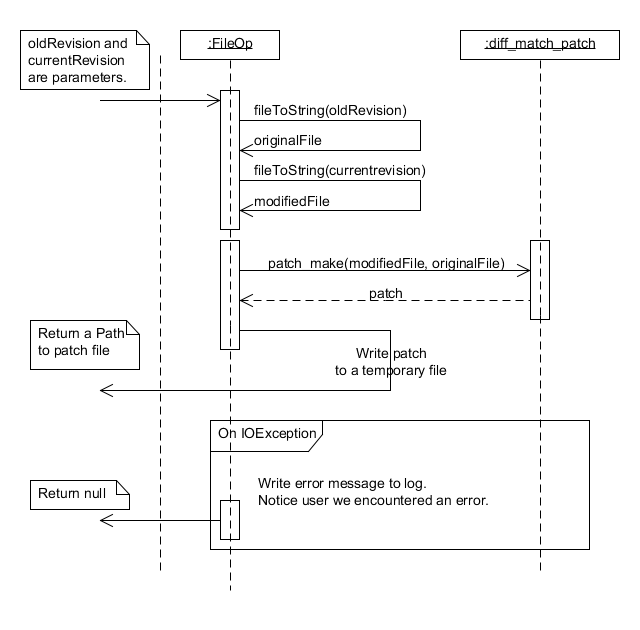
\includegraphics[width=\textwidth]{images/createPatch_sequence.png}

\subsubsection{FileHistory.getRevisionInfo}
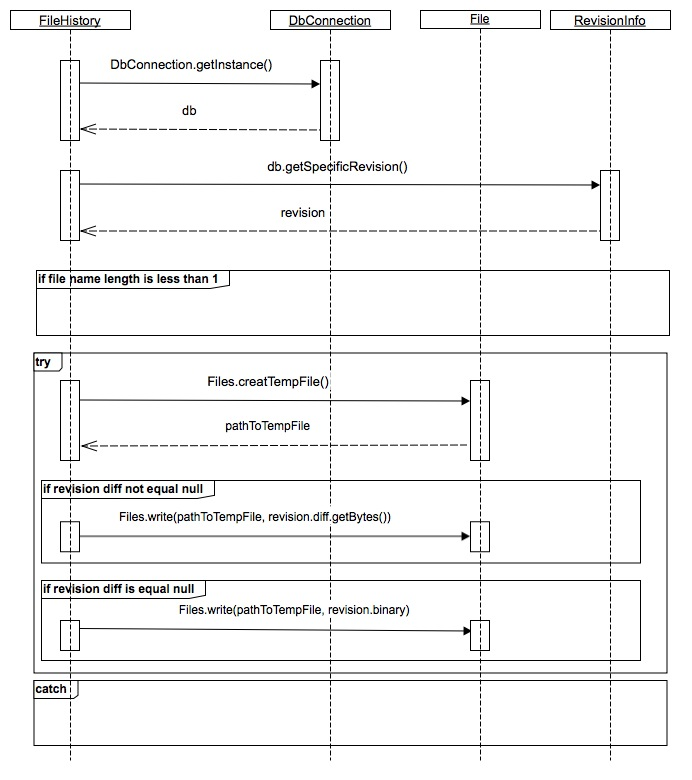
\includegraphics[width=\textwidth]{images/filehistory_getrivisioninfo-2.jpg}

\subsubsection{FileHistory.storeRevision}
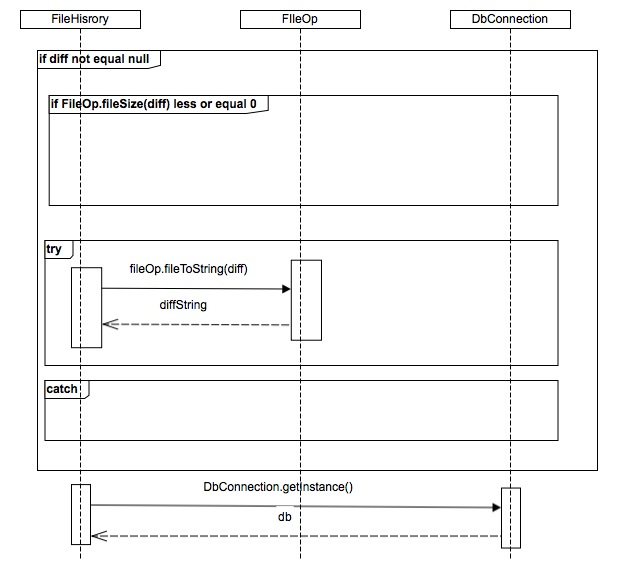
\includegraphics[width=\textwidth]{images/filehistory_storerevision.jpg}

\subsubsection{Startup.resolveBackupDirectory}
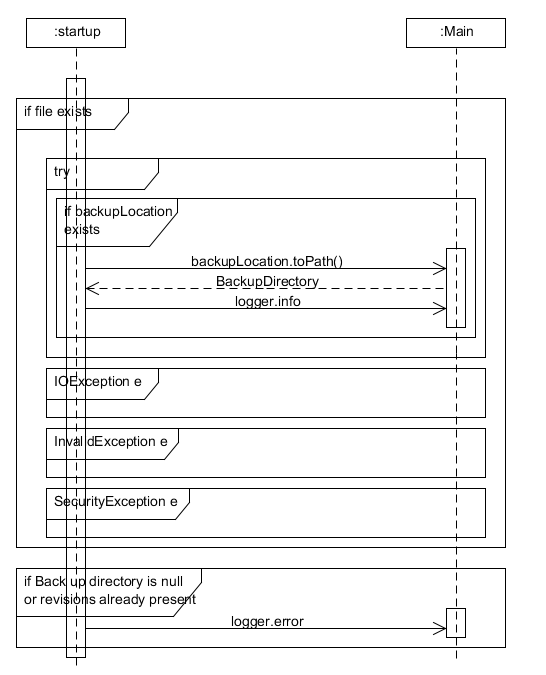
\includegraphics[width=\textwidth]{images/resolveBackupDirectory.png}

\subsubsection{DbConnection.getConfig}
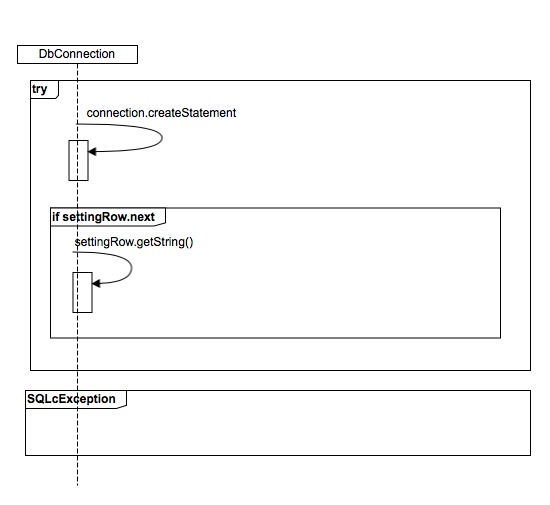
\includegraphics[width=\textwidth]{images/dbconnection_getconfig.jpg}

\subsection{Class diagram}
The class diagram is too large to embed in this document, so has been included separately as the file \texttt{class\_{}diagram.png}.

\subsection{Unit testing}

The test file is in \path{trunk/main/src/cmpt370/fbms/test}. TesterMainSuite.java is the test suite of the project.

The sample testing data is automatically created by test cases.\par
JUnit is also used in testing other modules, except the GUI modules, since the GUI modules are meant to be looked fine and no fault.

TTD is used while developing FileOp.  While developing, it decreased the weight of the class.

JUnit is a very powetful testing tool. It helps to avoid asserting in source code other than the test case, keeping the code clean. The setUp() and tearDown() eliminates the need to create and delete test samples, keeping the svn folder clean.

In all, JUnit is powerful to test base parts for a project. However, for GUI parts, we still need to review them by eyes.


\section{Re-engineering}

\subsection{Code smells}
Our project was found to have only two clones (both blind, with the latter also being classified as consistent). Preventing poor practices like clones was kept in mind when designing our program (and indeed, we probably removed several clones before we reached this point). We have no need to guess on why these clones appeared: we know why they exist.

\begin{longtable}{| p{1.5cm} | p{1.25cm} | p{12cm} |}
  \hline
  \textbf{ID} & \textbf{Root causes} & \textbf{Comments} \\ \hline
  40 \newline
  42 & 
  3.a(ii) \newline
  1.a(iv) &
  \textbf{FirstStartWizard.java lines 101-141 and 148-186} \tablepar
  Main reason is that abstraction here creates complexity. The two functions generate panels for the first start wizard. They need two different logging methods, two of the buttons need different labels, the panel text is different, and the values passed into two other functions are different. \tablepar
 The large number of differences would mean abstracting the problem into multiple functions would require a very large number of parameters, which ultimately ends up more confusing than the repetition. \\ \hline
 101 \newline
 102 &
 3.a(ii) \newline
 3.a(iv) &
 \textbf{MainMenu.java lines 148-176 181-210} \tablepar
 These two functions handle changing the backup and live directories, respectively. They're fairly similar except for the variables used to store the chosen path and the fact that they call different functions in their bodies. The latter is the reason for the clone. \tablepar
 These small methods weren't deemed worth the bother of implementing callbacks to handle the difference in their implementation. They're too specific and they are easier to understand without the necessary callback. \\ \hline
\end{longtable}

There are \textbf{no} clones in our project that cannot be refactored. All of our clones could be removed, we merely have deemed them not worth removing, for the reasons mentioned in the table.

There are some areas in our code, however, that resemble clones (but were not picked up by the clone detection software) and cannot be removed. In particular, the \texttt{TableSelecti\-onListener} and \texttt{RevisionTableSelectionListener} classes, located in \texttt{MainFrame.java} and \texttt{RevisionDialog.java}, respectfully, are quite similar at first look. With the exception of their constructors, they contain the same functions.

However, their behavior is quite different. They need to access variables in different ways to make all the necessary changes to the window (the table selector for the main frame, for example, has to disable menu options in the \texttt{MainMenu} object), one has to check if the selected row is a file or folder (whereas the other is selecting revisions which are assumed to exist in the database).

As an end result, there's a complicated network of dependencies and variances between those classes. They appear similar, but they just aren't compatible with each other and cannot be reliably merged while maintaining consistent functionality.

\subsection{Refactoring}
\begin{itemize}
\item We changed the static class \texttt{DbManager} into a singleton, and renamed it to \texttt{DbConnec\-tion}. In doing so, we set all the methods as non-static, added a private constructor, and added a \texttt{getInstance()} method.
\item We added helper method to handlers, which is \texttt{validateLists()} for clearing the lists, which lets us remove a vital dependency from  \texttt{GuiController}.
\item \texttt{Main} has become a singleton. This allows us to objectify \texttt{Watcher} and \texttt{GuiController} better, and decoupling the lists, which are no longer static.
\item \texttt{FileInfo} implemented \texttt{Comparible} to make comparisons between \texttt{FileInfo} objects considerably easier.
\item We renamed the \texttt{FileHistory}'s \texttt{obtainRevision()} method to \texttt{obtainRevisionCo\-ntent()}, which made the workings clearer and reduced confusion with the other methods in the class, which had similar names like \texttt{getRevision()} (which was renamed to \texttt{getRevisionInfo()}.

\item The if clauses in \texttt{DbConnection} (line 115 and 129) , \texttt{FilechangeHandlers} (line 57, 68, 79 and 90) and \texttt{Startup} (line 270) are reversed to enhance the readability.

\item Removed and consolidated rudundant code in \texttt{FileChangeHandlers} including common \texttt{FileOp} and \texttt{FileHistory} method call patterns. Putting them instead into class internal helper functions. 

\end{itemize}

\todonote{Butler, Tao, Alsharif, Rizvi. Everyone needs to point out at least one instance of refactoring, file and lines, why we did it, etc. Take a look at my objectification changes from revision 436 to 448 if you need ideas.}

\subsection{Gang of Four design patterns}
We used several Gang of Four design patterns in our project. One of the most notable is the use of a singleton for the \texttt{DbConnection} class. We used a singleton here because it's very slow to create and close connections at whim. The SQLite database manager we used supports serialized access, so the singleton is thread-safe.

The \texttt{FileOp} class, which performs file operations, is a facade. It provides easier access to modifications of the Java \texttt{Files} class and the libraries that we used. This makes the parameters and return values easier to work with and reduces the code present in other files. For example, we could copy a file with \texttt{Files.copy()}, but that doesn't handle directories well. \texttt{FileOp.copy()} cleanly handles both directories and files. It also allows us to just specify the directory to copy to, not the destination file name.

Or for another example, \texttt{isPlainText()} provides a simple way to get the MIME type from Java MIME magic and determine if the MIME type starts with ``text''. Without the use of \texttt{FileOp}, we'd be repeating a large block of code that is not as easily understood as ``is plain text''.

\section{Complete implementation and product delivery}

\subsection{Naming conventions}
In regards to naming conventions, our code roughly follows the \textit{Code Conventions for the Java language}\cite{conventions} as outlined by Sun.

\subsection{Commenting}
The FBMS project aims to be self documenting where possible. All functions and classes, however, are commented to explain their use, parameters, and return types.

\subsection{Pretty-printing of the source}
Instead of using some additional tool for formatting the source, we use the formatter built into Eclipse\cite{eclipse}. We configured the formatter to use our agreed upon conventions (a modified version of the \textit{Code Conventions for the Java language}\cite{conventions}) upon save.

Some of the differences include using tabs instead of spaces (for numerous reasons including consistency between editors and ease of use) and having braces start on a new line (making the opening braces easier to see).

\subsection{Usability engineering}
%% Place a figure with the settings image floating on the right somewhere in this
%% section (not necessarily at the top; going for best fit). Extra space at the top
%% and bottom are removed.
\begin{wrapfigure}{R}{0.5\textwidth}
\vspace{-20pt}
\begin{center}
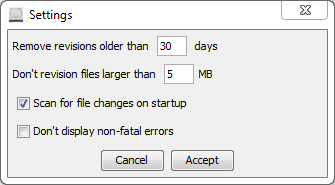
\includegraphics[width=0.48\textwidth]{images/settings.png}
\end{center}
\footnotesize{The settings dialog tries to phrase the options in a naturally readable manner and uses tooltips.}
\end{wrapfigure}

We designed FBMS to be easy to use and intuitive. The bulk of the user accessible portion of the program (ie, the GUI) is largely a file browser, so we looked at existing file browsers (such as Windows Explorer\cite{explorer} and Dolphin\cite{dolphin}) for design patterns. In particular, we changed the ``default'' behavior of the enter key in the file browser's table to activate the row instead of go to the next row. Similarly, rows are selected by single click and activated by double click.

In a number of places, we needed to prompt the user for paths (such as when choosing the live or backup directory). To make this more convenient, we supplied file chooser dialogs that only showed folders. We also skinned these dialogs to use the system dialog. So Windows users will see a Window-themed file chooser while Linx users would see an Linux themed file chooser.

The first run wizard was also intended to make the program much more usable. Instead of filling a configuration file or such, the user is guided through choosing the live and backup directories (or importing an existing backup) via a GUI wizard. This is not only more user friendly, but presents the opportunity to tell the user a bit about the program and how to use it.

To make the revision dialog more friendly, we added color based on whether a revision added or removed bytes. This dialog was inspired by the history pages of Wikipedia\cite{wikipedia}.

Finally, we included an option in the program's menu that opens up the documentation in their web browser.

\subsection{Complete implementation}
We have included the implementation in ``release'' and ``development'' versions.

The release version is pre-built and easy to use: just run the batch file (Windows) or shell script (Linux). This version is intended to allow the program to be run in a straightforward manner (allowing easy testing) and with optimal performance.

The development version does not contain pre-built binaries, but has the full source code available. To compile this, you will need Eclipse\cite{eclipse} or Ant\cite{ant}. This version is intended to allow the source code to be examined. Running the development program will be slower than the release version, since debugging is enabled and logging uses slower, more exact methods.

The release version is located in the \texttt{release} folder, relative to the location of this file. The development version is located in the \texttt{development} folder.

\todonote{Hoffert. Add the release and development folders (last minute)}

\subsection{User manual}
When the program is started for the first time, a wizard will guide you through selecting your live and backup directories.

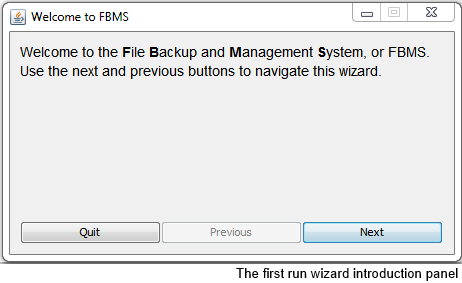
\includegraphics{images/1-firstRunIntro.png}
  
You can opt to start from scratch (specifying a backup and live directory), or import an existing backup directory (which will determine the live directory from previously saved settings).

\begin{itemize}
\item \textbf{Live directory:} The folder that you want to keep backed up and revisioned.
\item \textbf{Backup directory:} The location to store the backup. Don't use an existing folder, or you risk losing your files.
\end{itemize}

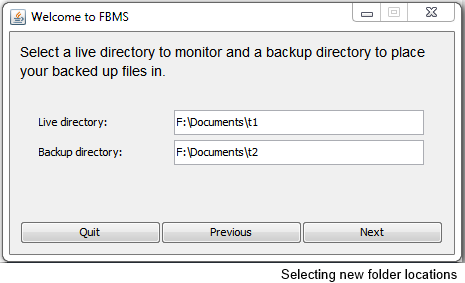
\includegraphics{images/2-newBackup.png}

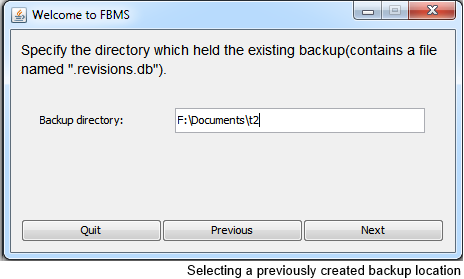
\includegraphics{images/3-oldBackup.png}

Once folders are chosen and the wizard is completed, the program will run quietly in the background. An icon will be created on the system tray. Double clicking this icon will open the program's interface.

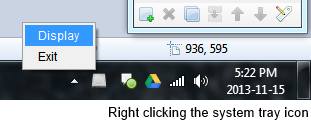
\includegraphics{images/4-systemTray.png}

The interface shows a special file browser, which displays the contents of the backup directory along with information such as the number of revisions stored. This file browser can be navigated with the keyboard or a mouse, and has functionality similar to other file browsers, such as Windows Explorer or Dolphin. It is, however, a specialized browser intended only to be able to restore files and view revisions.

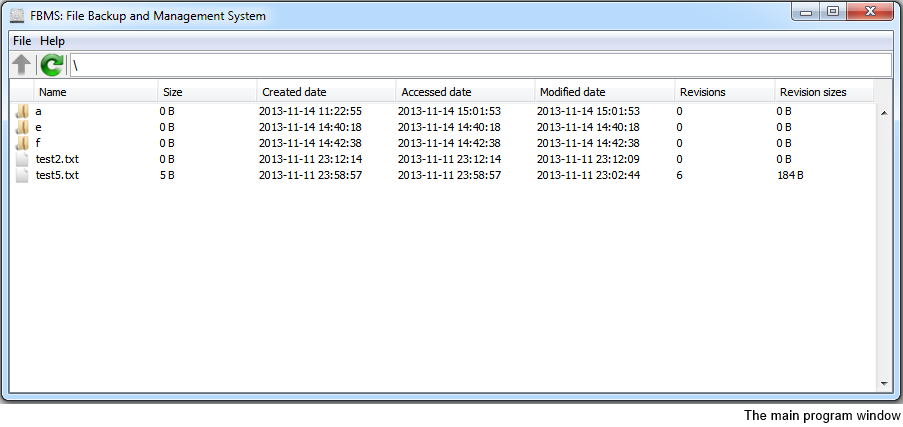
\includegraphics[width=\textwidth]{images/5-mainWindow.png}

Double clicking a file will open the revisions dialog, displaying a list of past revisions (if there are any). These revisions can be viewed (which opens the revision in your default program) or reverted (which sets that file in your live directory to the specified revision). You can also view the changes introduced by a revision, which will open in your default web browser.

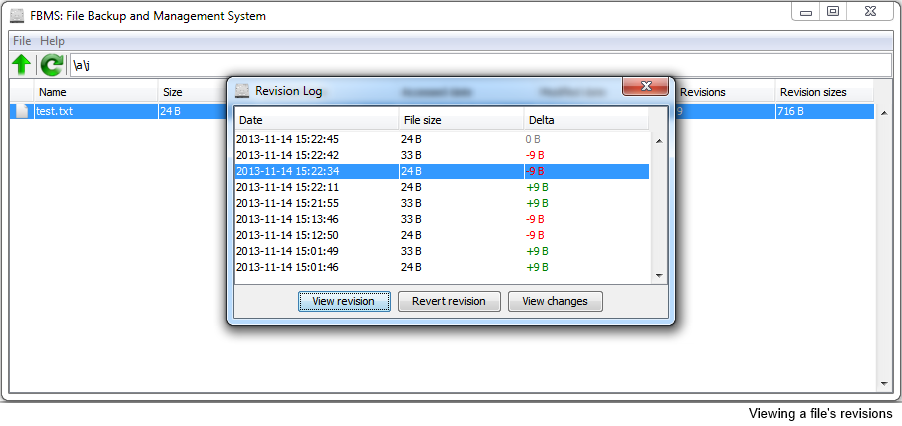
\includegraphics[width=\textwidth]{images/6-revisionDialog.png}

The file browser is also able to:

\begin{itemize}
\item Copy the selected file to a chosen folder
\item Restore all files
\item Change the live or backup directory
\end{itemize}

FBMS is also able to detect when files have changed since the last time you ran the program. When starting the program up, FBMS will perform a one time scan for file changes. This scan is slow, and can be disabled in the settings if FBMS is always running.

The settings dialog is accessed under the File menu of the GUI. It provides a few choices such as:

\begin{itemize}
\item Whether or not to display non-fatal error messages (which don't stop the program from running, but notify the user of issues).
\item Whether or not to run the previously mentioned first run scan
\item Whether or not to enable the trim feature, which removes revisions older than a specified date.
\end{itemize}

\section{Project plan, budget justification, and performance evaluation}
The following table breaks up the development of this milestone by group member. The time spent developing past milestones where contents was copied to this milestone is \textbf{not} included in this table.

%% The first column is a tiny little column for the section number.
%% The next column is the actual section name and subsection numbers.
%% Then we have the completed by column. Use \newline to create a new
%% paragraph line inside a table cell.
\begin{longtable}{| p{0.2cm} p{6.25cm} | p{3cm}| p{5cm} |}
  \hline
  \multicolumn{2}{|l|}{\textbf{List of tasks}} & \textbf{Completed by} & \textbf{Comments} \\ \hline
   & Abstract & Hoffert(0.1h) &  \\ \hline
  1. & Introduction &  &  \\ \hline
   & 1.1. System description & Hoffert(0.1h) &  \\ \hline
   & 1.2. Business case & Hoffert(0.1h) &  \\ \hline
   & 1.3. User-level goals & Hoffert(0.1h) &  \\ \hline
   & 1.4. User scenarios & Hoffert(0.1h) &  \\ \hline
   & 1.5. Scope document & Hoffert(0.1h) &  \\ \hline
   & 1.6. Project plan & Hoffert(0.2h) &  \\ \hline
   & 1.7. User involvement plan & Hoffert(0.1h) &  \\ \hline
   & 1.8. Low fidelity prototypes & Hoffert(0.25h) &  \\ \hline
  2. & Requirements and early design &  &  \\ \hline
   & 2.1. Summary use cases & Hoffert(2h)\newline Tao(1.5h) &  \\ \hline
   & 2.2. Fully-dressed use cases & Hoffert(0.5h) \newline Tao(0.5h) & Adapted to current design. \\ \hline
   & 2.3. Use case diagram & Tao(0.5h) &  \\ \hline
   & 2.4. Domain model &  &  \\ \hline
   & 2.5. Glossary & Hoffert(0.25h) &  \\ \hline
   & 2.6. Supplementary specification & Hoffert(0.25h) \newline Tao(0.5h) &  \\ \hline
   & 2.7. System sequence diagrams & Hoffert(0.5h) &  \\ \hline
   & 2.8. Operation contracts & Hoffert(1.5h)\newline Tao(1.5h) & \newline References of use cases  \\ \hline
   & 2.9. Obtaining user feedback & Hoffert(0.25h) &  \\ \hline
  3. & Updated design and unit testing &  &  \\ \hline
   & 3.1. System operations & Hoffert(0.25h) &  \\ \hline
   & 3.2. Sequence diagrams & Hoffert(2h) \newline Tao(3h) &  \\ \hline
   & 3.3. Class diagram & Hoffert(1.5h) &  \\ \hline
   & 3.4. Unit testing & Tao(0.5h) &  \\ \hline
  4. & Re-engineering &  &  \\ \hline
   & 4.1. Code smells & Hoffert(2h) &  \\ \hline
   & 4.2. Refactoring & Hoffert(0.25h) \newline Tao(1h) & \newline Refactored code \\ \hline
   & 4.3. Gang of Four design patterns & Hoffert(0.5h) &  \\ \hline
  5. & Complete implementation &  &  \\ \hline
   & 5.1. Naming conventions & Hoffert(0h) &  \\ \hline
   & 5.2. Commenting & Hoffert(0h) &  \\ \hline
   & 5.3. Pretty-printing & Hoffert(0.1h) &  \\ \hline
   & 5.4. Usability engineering & Hoffert(0.5h) &  \\ \hline
   & 5.5. Complete implementation & Hoffert(0.25h) &  \\ \hline
   & 5.6. User manual & Hoffert(0.1h) &  \\ \hline
  6. & Project plan, evaluation & Hoffert(0.5h) &  \\ \hline
  7. & Conclusion & Hoffert(0.25h) &  \\ \hline
  8. & Acknowledgements & Hoffert(0.25h) &  \\ \hline
   & References & Hoffert(0h) &  \\ \hline
    & \textbf{Total member contributions} & \textbf{Hoffert} & 14.35h \\ \cline{3-4}
    &  & \textbf{Tao} & 8.5h \\ \cline{3-4}
    &  & \textbf{Butler} & \\ \cline{3-4}
    &  & \textbf{Rizvi} & \\ \cline{3-4}
    &  & \textbf{Alsharif} & \\ \hline
    & \textbf{Grand total} &  & 22.85h \\ \hline
\end{longtable}

The next table summarizes the time spent by each member throughout the project (not including the time counted on the above table):

%% In this table, the first column is the member name (gonna wanna leave
%% that blank on subsequent rows for a member). Then we have the tasks
%% ("responsible for") column (overriden on the total row). Finally,
%% contributions and comments. This table will probably be cramped, so keep
%% it short and sweet.
\begin{longtable}{| p{2cm} | p{5cm} | p{3cm}| p{4.5cm} |}
  \hline
  \textbf{Group member} & \textbf{Responsible for} & \textbf{Contributions} & \textbf{Comments} \\ \hline
  Hoffert & Planning and documentation & 5 hours & Almost entire technical details document\\ \cline{2-4}
   & Previous milestones & 14 hours & \\ \cline{2-4}
   & Utility demo & 8 hours & Used to test features and toy demo in M2 \\ \cline{2-4}
   & Skeleton implementation and PoD classes & 2 hours & \\ \cline{2-4}
   & Watcher class & 1 hour & \\ \cline{2-4}
   & DbConnection.init() & 3 hours & \\ \cline{2-4}
   & FirstRunWizard & 6 hours & \\ \cline{2-4}
   & Data.getFolderContents() & 2 hours & Later renamed ``DataRetriever'' \\ \cline{2-4}
   & Various Control code related to startup & 5 hours & \\ \cline{2-4}
   & JUnit testing code & 4 hours & Most later revamped by Tao \\ \cline{2-4}
   & Errors class & 3 hours & \\ \cline{2-4}
   & MainFrame table & 5 hours & Table and listener dominantly my work \\ \cline{2-4}
   & MainMenu functionality & 2 hours & \\ \cline{2-4}
   & MainToolBar functionality & 1 hour & \\ \cline{2-4}
   & RevisionDialog table & 2 hours & \\ \cline{2-4}
   & SettingsDialog & 3 hours & \\ \cline{2-4}
   & Redid FileOp.createPatch and FileOp.applyPatch & 2 hours & Original library didn't work \\ \cline{2-4}
   & Data.getTableData and Data.getRevisionData & 3 hours & \\ \cline{2-4}
   & Data number formatting & 1 hour & With some third party code\\ \cline{2-4}
   & Trim database feature & 3 hours & \\ \cline{2-4}
   & FileOp utility functions & 2 hours & \\ \cline{2-4}
   & Refactoring & 4 hours & Objectification, use of design patterns \\ \cline{2-4}
   & Binary revisioning feature & 5 hours & Also lumped in bug fixes to file handlers \\ \cline{2-4}
   & MIME detection & 3 hours & Getting Java MIME Magic to work\\ \cline{2-4}
   & Usability fixes & 1 hour & As suggested by marker in M5 \\ \hline
   & Miscellaneous bug fixes & 4 hours & Numerous smaller bug fixes\\ \hline
  \multicolumn{2}{|r|}{\textbf{Total for Hoffert}} & 93 hours & 67\% of the commits from one person\\ \hline \hline
  Tao & Rough design of modules & 1 hour & \\ \cline{2-4}
   & Rough design of functions & 1 hour & \\ \cline{2-4}
   & Work on M1-M3 & 4 hours & \\ \cline{2-4}
   & Work on M4 text & 5 hours & \\ \cline{2-4}
   & Work on M4 graph & 2 hours & \\ \cline{2-4}
   & Work on FileOp & 7 hours & \\ \cline{2-4}
   & Revamping test case & 2 hours & \\ \cline{2-4}
   & FileOp test cases & 2 hours & \\ \cline{2-4}
   & FileChangeHandlers \newline test cases & 5 hours & \\ \cline{2-4}
   & Work on FileHistory & 6 hours & \\ \cline{2-4}
   & Redo operation contracts & 1 hours & \\ \cline{2-4}
   & Build.xml and run script & 4.5 hours & \\ \cline{2-4}
   & Work on M5 graph & 5 hours & \\ \cline{2-4}
   & Miscellaneous bug fixes & 2.5 hours & \\ \hline
  \multicolumn{2}{|r|}{\textbf{Total for Tao}}  & 48 hours & Preliminary design and library suggestion \\ \hline \hline
  Butler &  &  & \\ \cline{2-4}
   &  &  & \\ \cline{2-4}
   &  &  & \\ \cline{2-4}
   &  &  & \\ \hline
  \multicolumn{2}{|r|}{\textbf{Total for Butler}}  &  & \\ \hline \hline
  Rizvi &  &  & \\ \cline{2-4}
   &  &  & \\ \cline{2-4}
   &  &  & \\ \cline{2-4}
   &  &  & \\ \hline
  \multicolumn{2}{|r|}{\textbf{Total for Rizvi}}  &  & \\ \hline \hline
  Alsharif &  &  & \\ \cline{2-4}
   &  &  & \\ \cline{2-4}
   &  &  & \\ \cline{2-4}
   &  &  & \\ \hline
  \multicolumn{2}{|r|}{\textbf{Total for Alsharif}}  &  & \\ \hline
\end{longtable}

Our initial estimate focused largely on the ``basics'', the features we absolutely needed. However, we finished those and managed to add many extra features that weren't originally planned. The introduction estimated 150 man hours of work to create the system. The features mentioned in the introduction took 147 man hours including planning, testing, and debugging time, but not including time spent on the milestones.

This indicates that our estimate was very close. If we include the time spent on past milestones (not including this one), the total time comes to over 200 man hours. Another 15 man hours was needed to bring the program up to version 2.0, which consisted entirely of ``extra'' features. 

\todonote{Tao, Rizvi, Alsharif, Butler. Fill me out, yo!}

\section{Conclusion}
FBMS is a program that balances ease of use with power. It's geared at those wanting something inbetween the power of version control and the ease of use of online backup solutions. FBMS goes beyond most backup systems to store revisions of files. Monitoring the file system real time allowed efficiency for the system, which focuses on a single folder rather than an entire hard drive.

FBMS is best used for small projects where files change rapidly, where the system's live monitoring comes in handy. FBMS supports multi-drive systems, and works best when the backup and live directory are on different drives, decreasing the risk of losing both at the same time. 

\section{Acknowledgements}
\textbf{FBMS was created by:}
\begin{itemize}
\item Mike Hoffert (mlh374)
\item Da Tao (dat293)
\item Michael Butler (mdb815)
\item Ahsen Rizvi (sar457)
\item Hattan Alsharif (haa775)
\end{itemize}

\textbf{Some code derived from work by:}
\begin{itemize}
\item aioobe <\url{http://stackoverflow.com/users/276052/aioobe}>
\item erickson <\url{http://stackoverflow.com/users/3474/erickson}>
\end{itemize}

\textbf{Resources:}
\begin{itemize}
\item Program and refresh icons by oxygen (CC-BY-SA 3.0) \\
\url{http://www.oxygen-icons.org/}
\item Up icon by crystal (LGPL-2.1) \\
\url{http://www.everaldo.com/}
\item File and folder icons by nuovext2 (LGPL-2.1) \\
\url{http://nuovext.pwsp.net/}
\end{itemize}

\textbf{FBMS is licensed under GPL v3:} \\
\url{https://code.google.com/p/fbms} \\

\textbf{Log4j is licensed under the Apache License v2:} \\
\url{https://logging.apache.org/log4j/1.2/} \\

\textbf{SQLite JDBC Driver is licensed under the Apache License v2:} \\
\url{https://bitbucket.org/xerial/sqlite-jdbc} \\

\textbf{JNotify is licensed under the LGPL v2:} \\
\url{http://jnotify.sourceforge.net/} \\

\textbf{google-diff-match-patch is licensed under the Apache License v2:} \\
\url{https://code.google.com/p/google-diff-match-patch/} \\

\textbf{Java MIME Magic is licensed under GPL v2:} \\
\url{https://github.com/arimus/jmimemagic}

\begin{thebibliography}{9}

\bibitem{dropbox}
  Dropbox: \url{https://www.dropbox.com/}
  
\bibitem{svn}
  Subversion: \url{https://subversion.apache.org/}

\bibitem{git}
  Git: \url{http://git-scm.com/}

\bibitem{conventions}
  Code Conventions for the Java language: \url{http://www.oracle.com/technetwork/java/javase/documentation/codeconvtoc-136057.html}
  
\bibitem{eclipse}
  The Eclipse IDE: \url{http://www.eclipse.org/}

\bibitem{explorer}
  Windows Explorer on Wikipedia: \url{https://en.wikipedia.org/wiki/File_Explorer}

\bibitem{dolphin}
  Dolphin File Manager: \url{http://dolphin.kde.org/}
  
\bibitem{wikipedia}
  Example Wikipedia history page: \url{https://en.wikipedia.org/w/index.php?title=Software_engineering&action=history}
  
\bibitem{ant}
  Apache Ant: \url{https://ant.apache.org/}

\end{thebibliography}

\end{document}